\chapter{Opérations avec les nombres décimaux}\label{ChOpNbEntDec}

\begin{acquis}
\begin{itemize}
\item multiplier et diviser mentalement par 0,1; 0,01; 0,001; 10; 100; 1 000… des nombres décimaux et compléter les opérations à trous correspondantes;
\item soustraire, additionner et multiplier des nombres décimaux;
\item faire une division décimale par un diviseur entier et non entier avec un résultat exact ou un résultat à une précision donnée ou un résultat arrondi;
\item résoudre des problèmes dont la solution conduit à effectuer 2 ou 3 opérations successives parmi l’addition, la soustraction, la multiplication et la division de décimaux;
\item utiliser le vocabulaire suivant : somme, différence, produit, quotient, terme, facteur, dividende, diviseur et reste;
\end{itemize}
\end{acquis}

\cours
\section{Multiplier/diviser un nombre décimal par 10, 100, 1000}
%%%%%%%%%%%%%%%%%%%%%%%%%%%%%%%%%%%%%%%%%%%%%%%%%%%%%%%%%%%%%%%%%%%%%%%%%%%
\prof
{En primaire et de façon usuelle, on a l'habitude de parler de virgule qui se déplace. Cependant, pour coller à la réalité mathématiques, on préfèrera ici parler de quantité qui augment ou aui dimnue et donc de chiffres qui se déplacent. Cela n'empêche pas, une fois le concept acquis de montrer qu'on peut imaginer un déplcement de la virgule.}
%%%%%%%%%%%%%%%%%%%%%%%%%%%%%%%%%%%%%%%%%%%%%%%%%%%%%%%%%%%%%%%%%%%%%%%%%%%

\begin{aconnaitre}

\hspace{2em}\textbullet\hspace{.25em} Multiplier un nombre décimal par 10, 100 ou 1 000 revient à \textbf{\textcolor{C2}{déplacer chacun de ses chiffres vers la gauche}} de 1, 2 ou 3 rangs pour lui donner une valeur 10, 100 ou 1 000 fois plus grande.

\hspace{2em}\textbullet\hspace{.25em} Diviser un nombre décimal par 10, 100 ou 1 000 revient à \textbf{\textcolor{C2}{déplacer chacun de ses chiffres vers la droite}} de 1, 2 ou 3 rangs pour lui donner une valeur 10, 100 ou 1 000 fois plus petite.

\end{aconnaitre}

\begin{methode*1}[]
	\begin{remarque}
On devra parfois ajouter des zéros dans l'écriture.
	\end{remarque}
	\begin{exemple*1}

Effectuer les calculs $6,5 \div 100$ et $0,47 \times 1000$ [0.5em]

\begin{minipage}{.4\linewidth}
\begin{ttableau}{.8\linewidth}{4}
\hline
 \rotatebox{90}{unités} & \rotatebox{90}{dixièmes} & \rotatebox{90}{centièmes\phantom{x}} & \rotatebox{90}{millièmes} \\ \hline
 \textcolor{B1}{\textbf{6}} , & \textcolor{B1}{\textbf{5}} & & \\ \hline
 $0\,,$ & 0 & \textcolor{B1}{\textbf{6}} & \textcolor{B1}{\textbf{5}} \\ \hline
\end{ttableau}
\end{minipage}\hfill%
%
\begin{minipage}{.55\linewidth}
Pour diviser 6,5 par \textcolor{B1}{\textbf{100}}, on déplace chacun de ses chiffres vers la droite de \textcolor{B1}{\textbf{2}} rangs et on ajoute les zéros nécessaires. 

On obtient $6,5 \div 100 = 0,065$.

\end{minipage}
%

\vspace{2em}

\begin{minipage}{.4\linewidth}
\begin{ttableau}{\linewidth}{5}
\hline
\rotatebox{90}{centaines} & \rotatebox{90}{dixaines} & \rotatebox{90}{unités} & \rotatebox{90}{dixièmes} & \rotatebox{90}{centièmes\phantom{x}} \\ \hline
 & & 0 , & \textcolor{J1}{\textbf{4}} & \textcolor{J1}{\textbf{7}} \\ \hline
 \textcolor{J1}{\textbf{4}} & \textcolor{J1}{\textbf{7}} & 0 & &\\ \hline
\end{ttableau}
\end{minipage}\hfill%
%
\begin{minipage}{.55\linewidth}
Pour multiplier 0,47 par \textcolor{J1}{\textbf{1\,000}}, on déplace chacun de ses chiffres vers la gauche de \textcolor{J1}{\textbf{3}} rangs et on ajoute les zéros nécessaires. 

On obtient $0,47 \times 1\,000 = 470$. 
\end{minipage}
	\end{exemple*1}
	
\exercice

Compléter par le signe qui convient.
\begin{colenumerate}{4}
 \item $0,8 \dotfill 100=80$ ;
 \item $0,38 \dotfill 10=0,038$ ;
 \item $47 \dotfill 100=0,47$ ;
 \item $5 \dotfill 0,1=0,5$;
 \end{colenumerate}


\exercice

Effectue : 
\begin{colenumerate}{4}
 \item $3,6 \times 100$ ;
 \item $870 \times 1\,000$ ;
 \item $63 \div 10$ ;
 \item $87\,654 \div 100$.
 \end{colenumerate}
%\correction
 
\end{methode*1}








%%%%%%%%%%%%%%%%%%

\section{Multiplier/diviser un nombre décimal par 0,1 ; 0,01 ; 0,001}

\begin{aconnaitre}
\textbf{Multiplier} un nombre décimal par \textcolor{A1}{\textbf{0,1}}, \textcolor{B1}{\textbf{0,01}} ou \textcolor{J1}{\textbf{0,001}} revient à déplacer chacun de ses chiffres vers \textbf{la droite} de 1, 2 ou \textcolor{J1}{\textbf{3}} rangs pour lui donner une valeur 10, 100 ou \textcolor{J1}{\textbf{1\,000}} fois plus petite.
\textbf{Diviser} un nombre décimal par \textcolor{A1}{\textbf{0,1}}, \textcolor{B1}{\textbf{0,01}} ou \textcolor{J1}{\textbf{0,001}} revient à déplacer chacun de ses chiffres vers \textbf{la gauche} de \textcolor{A1}{\textbf{1}}, \textcolor{B1}{\textbf{2}} ou \textcolor{J1}{\textbf{3}} rangs pour lui donner une valeur \textcolor{A1}{\textbf{10}}, \textcolor{B1}{\textbf{100}} ou \textcolor{J1}{\textbf{1\,000}} fois plus grande.
\end{aconnaitre}


\begin{methode*1}[Multiplier ou diviser un nombre décimal par 0,1 ; 0,01 ; 0,001 \ldots]

\begin{remarque}
On devra parfois ajouter des zéros dans l'écriture.
\end{remarque}

\begin{exemple*1}
Effectue les calculs $2,5 \times 0,01$ et $0,65 \div 0,001$.\\[1em]

\begin{minipage}{.4\linewidth}
\begin{ttableau}{.8\linewidth}{4}
\hline
 \rotatebox{90}{unités} & \rotatebox{90}{dixièmes} & \rotatebox{90}{centièmes\phantom{x}} & \rotatebox{90}{millièmes} \\ \hline
 \textcolor{B1}{\textbf{2}} , & \textcolor{B1}{\textbf{5}} & & \\ \hline
 $0\,,$ & 0 & \textcolor{B1}{\textbf{2}} & \textcolor{B1}{\textbf{5}} \\ \hline
\end{ttableau}
\end{minipage}\hfill%
%
\begin{minipage}{.55\linewidth}
Pour multiplier 2,5 par \textcolor{B1}{\textbf{0,01}}, on déplace chacun de ses chiffres vers la droite de \textcolor{B1}{\textbf{2}} rangs et on ajoute les zéros nécessaires. 

On obtient $2,5 \times 0,01 = 0,025$.
\end{minipage}
%

\vspace{2em}

%
\begin{minipage}{.4\linewidth}
\begin{ttableau}{\linewidth}{5}
\hline
\rotatebox{90}{centaines} & \rotatebox{90}{dixaines} & \rotatebox{90}{unités} & \rotatebox{90}{dixièmes} & \rotatebox{90}{centièmes\phantom{x}} \\ \hline
 & & 0 , & \textcolor{J1}{\textbf{6}} & \textcolor{J1}{\textbf{5}} \\ \hline
 \textcolor{J1}{\textbf{6}} & \textcolor{J1}{\textbf{5}} & 0 & &\\ \hline
\end{ttableau}
\end{minipage}\hfill%
%
\begin{minipage}{.55\linewidth}
Pour diviser 0,65 par \textcolor{J1}{\textbf{0,001}}, on déplace chacun de ses chiffres vers la gauche de \textcolor{J1}{\textbf{3}} rangs et on ajoute les zéros nécessaires. 

On obtient $0,65 \div 0,001 = 650$.
\end{minipage}
\end{exemple*1}


\exercice

Effectuer :
\begin{colenumerate}{4}
 \item $5,45 \times 0,1$ ;
 \item $854 \times 0,001$ ;
 \item $63 \div 0,1$ ;
 \item $87,54 \div 0,01$.
 \end{colenumerate}
%\correction

\end{methode*1}

%%%%%%%%%%%%%%%%%%%%%%%%%%%%%%%%%%%%%%%%%%%%%%%%%%%%%%%%
\section{Multiplication}
\begin{remarque}

Multiplier c'est répéter la même quantité un certain nombre de fois.
\end{remarque}
	\subsection{Multiplier des décimaux}
\begin{aconnaitre}
Le résultat d'une multiplication s'appelle un produit. Les nombres que l'on multiplie sont des facteurs.
\end{aconnaitre}

\begin{methode*1}[Multiplication]
\begin{exemple*1}

$12 \times 4=48$

48 est le produit. 12 et 4 sont des facteurs.
\end{exemple*1}

\exercice

$13\times 3=39$

\dotfill est le \dotfill . \dotfill et \dotfill sont des \dotfill .

\end{methode*1}

	\subsection{Multiplier plusieurs facteurs}
\begin{aconnaitre}
Dans le calcul d'un produit de plusieurs facteurs, on peut:

\hspace{2em}\textbullet\hspace{.25em} changer l'ordre des facteurs.

\hspace{2em}\textbullet\hspace{.25em} regrouper différemment certains facteurs pour faciliter les calculs.
\end{aconnaitre}
\begin{methode*1}[]
\begin{exemple*1}

$25 \times 32 \times 4=25 \times 4 \times 32=100  \times 32 = 3200$
\end{exemple*1}

\exercice

$2 \times 3 \times 5= \dotfill$
\end{methode*1}
	
	\subsection{Multiplier deux nombres décimaux}
\begin{methode*1}[Multiplication de décimaux]
\begin{exemple*1}

Effectue la multiplication de 2,34 par 1,2.\\[0.5em]

On pose l'opération comme s'il s'agissait de nombres entiers. 

On effectue la multiplication de 234 par 12 sans tenir compte des virgules.

\begin{minipage}{.6\linewidth}
\begin{tabular}{rrrrcrrrr}
& 2, & 3 & 4 & $\xrightarrow{\times \text{\textcolor{B1}{\textbf{100}}}}$ & & 2 & 3 & 4 \\
$\times$ & & 1, & 2 & $\xrightarrow{\times \text{\textcolor{A1}{\textbf{10}}}}$ & $\times$ & & 1 & 2 \\ \cline{1-4} \cline{6-9}
& & & & & & 4 & 6 & 8 \\
& & & & & 2 & 3 & 4 & . \\ \cline{1-4} \cline{6-9}
2, & 8 & 0 & 8 & $\xleftarrow{\,\div\,\text{\textcolor{J1}{\textbf{1\,000}}}}$ & 2 & 8 & 0 & 8 \\
\end{tabular}
\end{minipage}\hfill%
%
\begin{minipage}{.37\linewidth}
234 est \textcolor{B1}{\textbf{100}} fois plus grand que 2,34 et 12 est \textcolor{A1}{\textbf{10}} fois plus grand que 1,2. Le produit $2,34 \times 1,2$ est donc \textcolor{J1}{\textbf{1\,000}} fois plus petit que 2\,808. Pour obtenir le résultat, on effectue donc $2\,808 \div 1\,000$.\\[0.75em]
\end{minipage}
Finalement $2,34 \times 1,2 = 2,808$.
\end{exemple*1}

\exercice

Sachant que $168 \times 32 = 5\,376$, détermine les produits (sans aucun calcul) :
\begin{colenumerate}{4}
 \item $168 \times 3,2$ ;
 \item $16,8 \times 0,32$ ;
 \item $1\,680 \times 3,2$ ;
 \item $1,68 \times 32$.
\end{colenumerate}
%\correction

Pose et effectue les opérations :
\begin{colenumerate}{4}
 \item $68,7 \times 39$ ;
 \item $123 \times 6,3$ ;
 \item $1,3 \times 0,7$ ;
 \item $54,6 \times 8,25$.
\end{colenumerate}
%\correction
\end{methode*1}

%%%%%%%%%%%%%%%%%%%%%%%%%%%%%%%%%%%%%%%%%%%%%%%%%%%%%%%%%%%%%%%%%%%%%%%%%%%  
\section{Division}
\begin{remarque}

Diviser c'est:
\begin{itemize}
\item partager une quantité en parts égales\\
OU
\item constituer des groupes de même taille
\end{itemize}
\end{remarque}
\begin{methode*1}[Diviser un nombre décimal par un nombre entier]

\begin{exemple*1}
Effectue la division de 75,8 par 4.\\[0.5em]

\begin{minipage}[c]{.26\textwidth}
\vspace{0em}
\begin{center}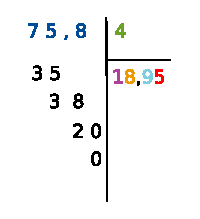
\includegraphics[width=3cm]{div758-4} \end{center}

\end{minipage}\hfill% 
\begin{minipage}[c]{.66\textwidth}

On commence par diviser la partie entière. On partage \textcolor{A1}{7} dizaines en \textcolor{H1}{4} ; le quotient comportera \textcolor{C1}{1} dizaine.\\[0.75em]
Il reste 3 dizaines. Avec les \textcolor{A1}{5} unités en plus, cela fait 35 unités à partager en \textcolor{H1}{4} ; le quotient comportera \textcolor{J1}{8} unités. \\[0.75em]
Il reste 3 unités soit 30 dixièmes. Avec les \textcolor{A1}{8} dixièmes en plus, cela fait 38 dixièmes à partager en \textcolor{H1}{4} ; le quotient comportera \textcolor{A3}{9} dixièmes. On doit donc écrire la virgule dans le quotient.\\[0.75em]
Il reste 2 dixièmes soit 20 centièmes (on a ajouté un zéro) à partager en \textcolor{H1}{4} ; le quotient comportera donc \textcolor{B2}{5} centièmes.\\[0.75em]
Ainsi $\textcolor{A1}{75,8} \div \textcolor{H1}{4} = \textcolor{C1}{1}\textcolor{J1}{8},\textcolor{A3}{9}\textcolor{B2}{5}$.
\end{minipage}

\end{exemple*1}

\exercice

Calcule la valeur exacte ou une valeur arrondie au centième des quotients :
\begin{colenumerate}{4}
 \item $10 \div 7$ ;
 \item $24,96 \div 8$ ;
 \item $5,2 \div 6$ ;
 \item $145,2 \div 3$.
 \end{colenumerate}
%\correction

\end{methode*1}

%%%%%%%%%%%%%%%%%%%%%%%%%%%%%%%%%%%%%%%%%%%%%%%%%%%%%%%%%%%%%%%%%%%%%%%%%%%

\begin{aconnaitre}
Le quotient de deux nombres \textbf{ne change pas} si on les multiplie (le dividende et le diviseur) par un même nombre non nul.
\end{aconnaitre}


\begin{methode*1}[Diviser un nombre décimal par un nombre décimal]

\begin{exemple*1}
Effectue la division de 32,4 par 2,25.\\[1em]
On commence par rendre entier le diviseur en le multipliant par 100 : $2,25 \times 100 = 225$. On multiplie le dividende par le même nombre : $32,4 \times 100 = 3\,240$. On effectue la division de 3\,240  par 226, soit $3\,240 \div 225 = 14,4$. On obtient ainsi le résultat de la division :

$32,4 \div 2,25 = 14,4$. 
\end{exemple*1}

\exercice

Calcule la valeur exacte ou une valeur arrondie au centième des quotients :
\begin{colenumerate}{4}
 \item $4 \div 6,37$ ;
 \item $13,4 \div 2,45$ ;
 \item $5,87 \div 2,3$ ;
 \item $0,84 \div 0,12$.
 \end{colenumerate}
%\correction

\end{methode*1}

%%%%%%%%%%%%%%%%%%%%%%%%%%%%%%%%%%%%%%%%%%%%%%%%%%%%%%%%%%%%%%%%%%%%%%%%%%%        



\exercicesbase
\begin{colonne*exercice}
 \definecolor{fondTI}{HTML}{869286}
%%%%%%%%%%%%%%%%%%%%%%%%%%%%%%%%%%%%%%%%%%%%%%%%%%%%%%%%%%%%%%%%%%%%%%%%%%%
\serie{Techniques opératoires}
\begin{exercice}
Calcule mentalement les additions :
\begin{enumerate} 
 \item $4,6 + 5,2$ \dotfill ; 
 
 \item $6,2 + 3,4$ \dotfill ; 
 
 \item $4,5 + 6,1$ \dotfill ; 
 
 \item $8,3 + 9,6$ \dotfill ; 
 
 \item $8 + 1,5$ \dotfill ; 
 
 \item $8,6 + 8,9$ \dotfill ; 
 
 \item $3,9 + 5,4$ \dotfill ; 
 
 \item $6,5 + 8,7$ \dotfill ; 
 
 \item $6,8 + 9,4$ \dotfill ; 
 
 \item \hspace{0.1em} $12,9 + 15,8$ \dotfill. 
 \end{enumerate}
\end{exercice}
\begin{exercice}
Calcule mentalement les soustractions :
\begin{enumerate} 
 \item $6,5 - 4,3$ \dotfill ; 
 
 \item $7,6 - 0,4$ \dotfill ; 
 
 \item $4,9 - 4,3$ \dotfill ; 
 
 \item $5,7 - 0,4$ \dotfill ; 
 
 \item $4,7 - 4,3$ \dotfill ; 
 
 \item $6,2 - 4,6$ \dotfill ; 
 
 \item $9 - 8,7$ \dotfill ; 
 
 \item $3,1 - 1,8$ \dotfill ; 
 
 \item $7,8 - 6,9$ \dotfill ; 
 
 \item \hspace{0.2em}$17,4 - 8,7$ \dotfill. 
 
 \end{enumerate}  
\end{exercice}
\begin{exercice}
Calcule les sommes en effectuant des regroupements astucieux :
\begin{enumerate} 
 \item $6,5 + 12,6 + 1,5$ ;
 \item $36,99 + 45,74 + 2,01 + 13,26$ ;
 \item $9,25 + 8,7 + 5,3 + 16,75$ ;
 \item $34,645 + 34,75 + 2,25 + 4,355$ ;
 \item $7,42 + 4,2 + 7,8 + 25,58$ ;
 \item $3,01 + 2,9 + 6,1 + 7,99 + 2,001$.
 \end{enumerate}
\end{exercice}
\begin{exercice}
Pose et effectue :
\begin{enumerate} 
 \item $853,26 + 4 038,3$ ;
 \item $52 + 8,63 + 142,8$ ;
 \item $49,3 + 7,432 + 12,7$ ;
 \item $948,25 - 73,2$ ;
 \item $9,8 - 0,073$ ;
 \item $83 - 43,51$.
 \end{enumerate} 
 \end{exercice}
\begin{exercice}
Calcule mentalement :
\begin{enumerate} 
 \item $435,7 \times 0,1$ \dotfill ; 
 
 \item $18,73 \times 0,01$ \dotfill ; 
 
 \item $439,345 \times 0,001$ \dotfill ; 
 
 \item $0,28 \times 0,1$ \dotfill ; 
 
 \item $39 \times 0,001$ \dotfill ; 
 
 \item $0,8 \times 0,01$ \dotfill ; 
 
 \item $354 \times 0,001$ \dotfill ; 
 
 \item $0,03 \times 0,001$ \dotfill. 
 
 \end{enumerate}
\end{exercice}
\begin{exercice}
Calcule mentalement :
\begin{enumerate} 
 \item $48 \div 0,1$ \dotfill ; 
 
 \item $12,97 \div 0,01$ \dotfill ; 
 \item $12,3 \div 0,001$ \dotfill ; 
 
 \item $0,45 \div 0,1$ \dotfill ; 
        
 \item $5,61 \div 0,0001$ \dotfill ; 
        
 \item $0,056 \div 0,1$ \dotfill ; 
 
 \item $354 \div 0,001$ \dotfill ; 
 
 \item $0,5 \div 0,001$ \dotfill. 
 \end{enumerate}
\end{exercice}
\begin{exercice}
Complète par le signe opératoire qui convient :
\begin{colenumerate}{2}
 \item $0,8 \ldots 100 = 80$ ;
 \item $0,38 \ldots 10 = 0,038$ ;
 \item $47 \ldots 100 = 0,47$ ;
 \item $380 \ldots 10 = 38$ ;
 \item $5 \ldots 0,1 = 0,5$ ;
 \item $60\,000 \ldots 10 = 6\,000$ ;
 \item $4\,100 \ldots 100 = 4\,000$ ;
 \item $5\,600 \ldots 100 = 56$ ;
 \item $8 \ldots 0,01 = 0,08$ ;
 \item \hspace{0.25em}$100 \ldots 1,2 = 120$.
 \end{colenumerate} 
\end{exercice}
\begin{exercice}
Calcule mentalement en détaillant ta démarche :
\begin{enumerate} 
 \item $0,1 \times 14 \times 1\,000$ \dotfill ; 
 
 \item $2,18 \times 0,001 \times 100$ \dotfill ; 
 \item $1,8 \times 0,01 \times 10$ \dotfill ; 
 \item $4 •\times 0,01 \times 100$ \dotfill. 
 \end{enumerate} 
\end{exercice}
\begin{exercice}
Sachant que $48 \times 152 = 7\,296$, détermine les résultats des calculs :
\begin{enumerate} 
 \item $48 \times 1,52$ \dotfill ; 
 
 \item $4,8 \times 15,2$ \dotfill ; 
 
 \item $0,48 \times 0,152$ \dotfill ; 
 
 \item $0,048 \times 1\,520$ \dotfill. 
 \end{enumerate} 
\end{exercice}
\begin{exercice}
Calcule en regroupant astucieusement :
\begin{enumerate} 
 \item $0,8 \times 2 \times 0,6 \times 50$ \dotfill ; 
 
 \item $0,25 \times 12,38 \times 4$ \dotfill ; 
 
 \item $8 \times 49 \times 1,25$ \dotfill ; 
 
 \item $2,5 \times 12,9 \times 0,04$ \dotfill ; 
 
 \item $0,15 \times 70 \times 0,02$ \dotfill ; 
 
 \item $75 \times 0,06 \times 0,4$ \dotfill. 
 
 \end{enumerate} 
\end{exercice}
\begin{exercice}
Place correctement la virgule dans le résultat de la multiplication (en ajoutant éventuellement un ou des zéros) :
\begin{enumerate} 
 \item $12,8 \times  5,3 = \textcolor{PartieGeometrie}{6\,784}$ ;
 \item $28,7 \times 1,04 = \textcolor{PartieGeometrie}{29\,848}$ ;
 \item $0,15 \times 6,3 = \textcolor{PartieGeometrie}{945}$ ;
 \item $0,008 \times 543,9 = \textcolor{PartieGeometrie}{43\,512}$ ;
 \item $0,235 \times 0,132 = \textcolor{PartieGeometrie}{3\,102}$.
 \end{enumerate}
\end{exercice}
\begin{exercice}
Pose et effectue les produits :
\begin{enumerate} 
 \item $2,08 \times 4,23$ \dotfill ; 
 
 \item $4,38 \times 5,7$ \dotfill ; 
 
 \item $6,93 \times 15,8$ \dotfill ; 
 
 \item $8,35 \times 0,18 $\dotfill.  
 \end{enumerate}
\end{exercice}
\begin{exercice} 
Calcule mentalement :
\begin{colenumerate}{2}
 \item $ 8,6 \div 2$ ;
 \item $ 24,8 \div 4$ ;
 \item $ 8,8 \div 8$ ;
 \item $ 7,7 \div 11$ ;
 \item $ 15,6 \div 3$ ;
 \item $ 63,6 \div 6$.
 \end{colenumerate}
\end{exercice}
\begin{exercice} 
Pose et effectue les divisions suivantes pour en trouver le quotient décimal exact :
\begin{enumerate} 
 \item $ 12,6 \div 6$ \dotfill ; 
 
 \item $ 28,48 \div 4$ \dotfill ; 
 \item $ 169,2 \div 3$ \dotfill ; 
 \item $ 0,162 \div 9$ \dotfill ; 
 \item $ 67,5 \div 4$ \dotfill ; 
 \item $ 9,765 \div 15$ \dotfill. 
 \end{enumerate}
\end{exercice}
\begin{exercice}[Valeurs approchées]
\vspace{-1em}
\begin{enumerate} 
 \item Pose et effectue les divisions suivantes jusqu'au millième :
 \begin{itemize}
  \item $12 \div 7$ \dotfill ; 
  
  \item $148,9 \div 12$ \dotfill ; 
  
  \item $13,53 \div 3$ \dotfill. 
  \end{itemize}
 \item Pose et effectue les divisions suivantes jusqu'au centième :
  \begin{itemize}
  \item $123,8 \div 7$ \dotfill ; 
  
  \item $235,19 \div 11$ \dotfill ; 
  
  \item $0,14 \div 3$ \dotfill. 
  \end{itemize}
 \end{enumerate}
\end{exercice}
\begin{exercice} 
Calcule la valeur exacte ou une valeur arrondie au centième des divisions suivantes :
\begin{enumerate} 
 \item $1 \div 2,74$ \dotfill ; 
 \item $5,87 \div 2,3$ \dotfill ; 
 \item $3,24 \div 1,7$ \dotfill ; 
 \item $45,6 \div 0,24$ \dotfill ; 
 \item $20,35 \div 8,5$ \dotfill ; 
 \item $0,53 \div 0,17$ \dotfill. 
 \end{enumerate}
\end{exercice}
\begin{exercice} 
Calcule la valeur exacte ou une valeur arrondie au centième des divisions suivantes :
\begin{enumerate} 
 \item $3,35 \div 0,42$ \dotfill ; 
 \item $41,5 \div 3,14$ \dotfill ; 
 \item $ 0,03 \div 2,1$ \dotfill ; 
 \item $0,35 \div 0,25$ \dotfill ; 
 \item $0,53 \div 0,8$ \dotfill ; 
 \item $21,7 \div 0,14$ \dotfill. 
 \end{enumerate}
\end{exercice}
%%%%%%%%%%%%%%%%%%%%%%%%%%%%%%%%%%%%%%%%%%%%%%%%%%%%%%%%%%%%%%%%%%%%%%%%%%%
%%%%%%%%%%%%%
\serie{Techniques opératoires}
\begin{exercice}
Calcule mentalement :
\begin{enumerate} 
 \item $4,357 \times 100$ \dotfill ; 
 
 \item $89,7 \times 1\,000$ \dotfill ; 
 
 \item $0,043 \times 10$ \dotfill ; 
 
 \item $0,28 \times 1\,000$ \dotfill ; 
 
 \item $39 \times 100$ \dotfill ; 
 
 \item $0,48 \times 10$ \dotfill ; 
        
 \item $354 \times 10$ \dotfill ; 
        
 \item $0,03 \times 10\,000$ \dotfill ; 
 
 \end{enumerate}
\end{exercice}
\begin{exercice}
Calcule mentalement :
\begin{enumerate} 
 \item $4\,338 \div 10$ \dotfill ; 
 
 \item $1\,297 \div 1\,000$ \dotfill ; 
        
 \item $12,3 \div 10$ \dotfill ; 
 
 \item $0,87 \div 100$ \dotfill ; 
        
 \item $3,8 \div 1\,000$ \dotfill ; 
 
 \item $0,04 \div 100$ \dotfill ; 
        
 \item $354 \div 10$ \dotfill ; 
 
 \item $12,5 \div 100$ \dotfill. 
 
 \end{enumerate}
\end{exercice}
\begin{exercice}
Complète par 10 ; 100 ; 1\,000 ; 10\,000 \ldots :
\begin{enumerate} 
 \item $8,79 \times \dotfill = 87,9$ ; 
 
 \item $4,35 \times \dotfill = 43\,500$ ; 
 
 \item $0,837 \times \dotfill = 8,37$ ; 
 
 \item $0,367 \times \dotfill = 3,67$ ; 
 
 \item $0,028 \times \dotfill = 0,28$ ; 
 
 \item $0,17 \div \dotfill = 0,017$ ; 
 
 \item $23 \div \dotfill = 0,23$ ; 
 
 \item $480 \div \dotfill = 4,8$ ; 
 
 \item $900 \div \dotfill = 0,09$ ; 
 
 \item \hspace{0.25em}$18\,000 \div \dotfill = 18$. 
 
 \end{enumerate}
\end{exercice}
\begin{exercice}
Place la virgule dans le nombre écrit en \textcolor{BleuOuv}{bleu} pour que l'égalité soit vraie :
\begin{enumerate} 
 \item $3,42 \times \textcolor{BleuOuv}{271} = 9,268\,2$ ;
 \item $\textcolor{BleuOuv}{432} \times 0,614 = 26,524\,8$ ;
 \item $0,48 \times \textcolor{BleuOuv}{62} = 29,76$ ;
 \item $2,6 \times \textcolor{BleuOuv}{485} = 126,1$ ;
 \item $\textcolor{BleuOuv}{45} \times 29,232 = 131,544$.
 \end{enumerate}
\end{exercice}
\begin{exercice}
Pose et effectue les produits :
\begin{enumerate} 
 \item $2,08 \times 4,23$ \dotfill ; 
 
 \item $4,38 \times 5,7$ \dotfill ; 
 
 \item $6,93 \times 15,8$ \dotfill ; 
 
 \item $8,35 \times 0,18 $\dotfill.  
 \end{enumerate}
\end{exercice}

\end{colonne*exercice}


\exercicesappr
\begin{colonne*exercice}
\begin{exercice}
Antoine possédait 832,25 CHF sur son livret d'épargne. Pour son anniversaire, ses parents y ont déposé 75 CHF. Combien a-t-il maintenant sur son livret ?
\end{exercice}


\begin{exercice}
Un panier plein de fruits pèse 1,836 kg. Vide, il pesait 0,425 kg. Quelle est la masse des fruits contenus dans ce panier ?
\end{exercice}


\begin{exercice}
Pierre a relevé le compteur de sa voiture au départ et au retour de vacances. Au départ, le compteur indiquait 58\,257,6 km. Au retour, il indiquait 59\,329,1 km. Quelle distance a‑t‑il parcourue pendant ses vacances ?
\end{exercice}


\begin{exercice}
Simon veut acheter un livre. Il a 25,35 CHF dans son porte‑monnaie et il lui manque 5,25 CHF pour acheter ce livre. Quel est le prix du livre ?
\end{exercice}


\begin{exercice}
Une voiture consomme 8,5 l d'essence pour faire 100 km. Combien d'essence consomme‑t‑elle pour faire 500 km ?
\end{exercice}
  
  
\begin{exercice}
Un employé gagne 17,25 CHF de l'heure. Il travaille 35 heures par semaine. Combien gagne‑t‑il chaque semaine ?
\end{exercice}


\begin{exercice}
Au marché, Anne a déposé dans son panier 1,2 kg de carottes, 600 g de raisin et 1,3 kg de pommes. Combien pèse le contenu de son panier ?
\end{exercice}


\begin{exercice}
Pour aller au collège, Caroline fait 1,4 km avec son vélo qu'elle laisse chez sa grand‑mère. Puis elle parcourt 150 m à pied jusqu'au collège. Quelle distance totale parcourt‑elle pour se rendre au collège ?
\end{exercice}


\begin{exercice}
Djamel a acheté 1,6 kg de poires à 2,30 CHF le kg. Combien a‑t‑il payé ?
\end{exercice}


\begin{exercice}
Gérard a payé 41,40 CHF pour 12 pieds de tomate. Quel est le prix d'un pied de tomate ?
\end{exercice}



\begin{exercice}
Un lot de six stylos identiques coûte 8,10 CHF. Quel est le prix d'un stylo ?
\end{exercice}


\begin{exercice}
Mercredi après‑midi, Anh Hao a fait cinq tours d'un circuit de VTT. Il a parcouru en tout 23,5 km. Quelle est la longueur de ce circuit ?
\end{exercice}


\begin{exercice}
Mme Betty possède 6,6 litres de jus de pomme. Combien de bouteilles de 0,7 litres pourra-t-elle remplir ?
\end{exercice}

\begin{exercice}
Agan possède 37,40 CHF en pièces de 20 centimes. Combien de pièces de 20 centimes possède t'il ?
\end{exercice}


\begin{exercice}[Calculer sans poser]


\begin{enumerate}
 \item Calcule mentalement les produits suivants sachant que $6,5 \times 3,7 = 24,05$ :
 \begin{colitemize}{3}
  \item $6,5 \times 37$ ;
  \item $65 \times 37$ ;
  \item $6,5 \times 0,37$ ;
  \item $0,65 \times 3,7$ ;
  \item $6\,500 \times 0,003\,7$ ;
  \item $65 \times 0,37$.
  \end{colitemize}
  
 \item Sachant que $935 \div 17 = 55$, que dire des quotients suivants ? Justifie.   
 \begin{colitemize}{2}
  \item $9 350 \div 170$ ;
  \item $93,5 \div 1,7$ ;
  \item $93\,500 \div 1\,700$ ;
  \item $9,35 \div 0,17$.
  \end{colitemize}
 \end{enumerate}
\end{exercice}


\begin{exercice}[Calculer sans poser (bis)]

\begin{enumerate}
 \item Calcule $96,5 + 83,7$ et $96,5 - 83,7$ ;
 \item Déduis‑en les sommes et les différences suivantes sans poser les opérations :
 \begin{colitemize}{2}
  \item $965 + 837$ ;
  \item $0,965 + 0,837$ ;
  \item $9,65 - 8,37$ ;
  \item $96\,500 - 83\,700$.
  \end{colitemize}
 \item Peut‑on trouver par ce moyen les résultats des opérations $96\,500 + 8\,370$ et $9\,650 - 837$ ? Pourquoi ?
 \end{enumerate}
\end{exercice}


\begin{exercice}[Que de restes !]

Dans une planche de 478,8 cm de long, on veut découper des étagères de 9 cm de long.
\begin{enumerate}
 \item Combien d'étagères peut‑on découper ? 

Quelle est la longueur du morceau restant ? 

\begin{center} 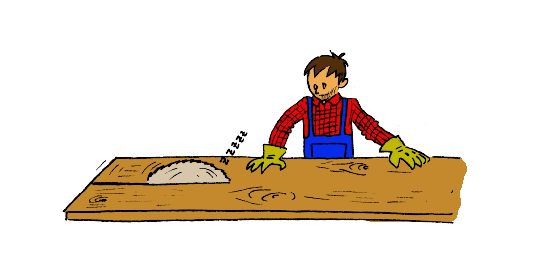
\includegraphics[width=5cm]{menuisier} \end{center}

Complète alors l'égalité $478,8 = 9 \times \ldots + \ldots$ . \label{NbEntDec_Approf81Qa}

 \item En utilisant la division écrite au \ref{NbEntDec_Approf81Qa}, recopie et complète les égalités suivantes :
 \begin{itemize}  
  \item $47,88 = 9 \times 5,3 + \ldots$ ;
  \item $4 788 = 9 \times 532 + \ldots$ ;
  \item $4 788 = 90 \times 53 + \ldots$ ;
  \item $4,788 = 9 \times \ldots + 0,018$.
  \end{itemize}
 \end{enumerate}
\end{exercice}


\begin{exercice}[Paquets empilés]
On a reçu au collège 7 rames de 500 feuilles pour la photocopieuse et 3 paquets de 24 pièces de « carton plume » :
\begin{enumerate}
 \item L'épaisseur d'une feuille de papier pour photocopieuse est de 0,11 mm et celle d'une pièce de « carton plume » est de 5 mm. Calcule un ordre de grandeur de la hauteur totale de tous ces paquets empilés ;
 \item Écris la hauteur totale des paquets en une seule expression puis calcule‑la.
 \end{enumerate}
\end{exercice}


\begin{exercice}[Densité de population]
On considère le tableau suivant :

\begin{center}
\begin{tabularx}{\linewidth}{|c|*{6}{>{\centering \arraybackslash}X|}}
\hline \rowcolor{U1} Continent & Nombre d'habitants & Superficie en km\up{2} \\
\hline \rowcolor{A3} Afrique & 965 millions & 30\,206\,704 \\
\hline \rowcolor{A3} Amérique & 911 millions & 42\,189\,120 \\
\hline \rowcolor{A3} Asie & 4,03 milliards & 43\,810\,582 \\
\hline \rowcolor{A3} Europe & 731 millions & 10\,180\,000 \\
\hline \rowcolor{A3} Océanie & 34 millions & 9\,008\,458 \\
\hline
\end{tabularx} \\
\end{center}

\begin{enumerate}
 \item Quel est le continent qui a le plus grand nombre d'habitants ? Et le plus petit nombre ?
 \item Quel est le continent qui a la plus grande superficie ? Et la plus petite ? 
 \end{enumerate}
\end{exercice}




\end{colonne*exercice}

\connaissances

\QCMautoevaluation{Pour chaque question, plusieurs réponses sont proposées. Déterminer celles qui sont correctes.} 

\begin{QCM}
  \begin{GroupeQCM} 
    \begin{exercice}
      Dix-huit millions huit cents s'écrit :
      \begin{ChoixQCM}{4}
      \item 18\,800\,000
      \item 18\,000\,800
      \item 18\,800
      \item 18\,008\,100
      \end{ChoixQCM}
\begin{corrige}
     \reponseQCM{b} 
   \end{corrige}
    \end{exercice}

    \begin{exercice}
      45 centaines est égal à :
      \begin{ChoixQCM}{4}
      \item 5 unités
      \item 450 dizaines
      \item 4 dizaines
      \item 45\,100
      \end{ChoixQCM}
      \begin{corrige}
     \reponseQCM{b}
   \end{corrige}
    \end{exercice}

    
    \begin{exercice}
      Un centième est :
      \begin{ChoixQCM}{4}
      \item plus grand qu'un dixième
      \item égal à dix millièmes
      \item plus petit qu'un millième
      \item égal à dix  dixièmes
      \end{ChoixQCM}
      \begin{corrige}
     \reponseQCM{b}
   \end{corrige}
    \end{exercice}


    \begin{exercice}
      Une écriture décimale de 456 centièmes est :
      \begin{ChoixQCM}{4}
      \item 456,100
      \item 456\,100
      \item 4,56
      \item 4\,560 millièmes
      \end{ChoixQCM}
      \begin{corrige}
     \reponseQCM{cd}
   \end{corrige}
    \end{exercice}


    \begin{exercice}
      Le nombre $5 + 0,4 + 0,007$ peut aussi s'écrire :
      \begin{ChoixQCM}{4}
      \item 547 millièmes
      \item 5,47
      \item 5,407
      \item 5\,047 millièmes
      \end{ChoixQCM}
      \begin{corrige}
     \reponseQCM{c}
   \end{corrige}
    \end{exercice}
 
       \begin{exercice}
      7 unités, 8 centièmes et 5 millièmes s'écrit :
      \begin{ChoixQCM}{4}
      \item 7,85
      \item 7,085
      \item 7,800\,500\,0
      \item 7,0085\,0
      \end{ChoixQCM}
      \begin{corrige}
     \reponseQCM{b}
   \end{corrige}
    \end{exercice}


     \begin{exercice}
      Un nombre compris entre 24,56 et 24,57 est par exemple...
      \begin{ChoixQCM}{4}
      \item 24\,568 millièmes
      \item 24,560\,7
      \item impossible, il n'y a pas de nombre compris entre 24,56 et 24,57
      \item $24 + 0,562$
      \end{ChoixQCM}
      \begin{corrige}
     \reponseQCM{abd}
   \end{corrige}
    \end{exercice}
    
     \begin{exercice}
      L'arrondi de 123,254 au dixième est...
      \begin{ChoixQCM}{4}
      \item 120
      \item 123,2
      \item 123,26
      \item 123,3
      \end{ChoixQCM}
      \begin{corrige}
     \reponseQCM{d}
   \end{corrige}
    \end{exercice}

     \begin{exercice}
      873,023 est ...
      \begin{ChoixQCM}{4}
      \item 1\,000 fois plus grand que 873\,230
      \item 100 fois plus petit que 87\,302,3
      \item 10\,000 fois plus grand que 0,087\,302\,3
      \item 10 fois plus petit que 87,302\,3
      \end{ChoixQCM}
      \begin{corrige}
     \reponseQCM{bc}
   \end{corrige}
    \end{exercice}
    
     \begin{exercice}
      $57,41 - 27,83 =$ ...
      \begin{ChoixQCM}{4}
      \item 30.42
      \item 30.58
      \item 29.58
      \item 19.58
      \end{ChoixQCM}
      \begin{corrige}
     \reponseQCM{c}
   \end{corrige}
    \end{exercice}


     \begin{exercice}
      $872,967 =$ ...
      \begin{ChoixQCM}{4}
      \item $87\,296,7 \div 100$
      \item $862,967 \times 10$
      \item $87,296\,7 \times 10$
      \item $8,729\,67 \times 100$
      \end{ChoixQCM}
      \begin{corrige}
     \reponseQCM{acd}
   \end{corrige}
    \end{exercice}
\end{GroupeQCM}
\end{QCM}

\begin{QCM}
\begin{GroupeQCM}
    
     \begin{exercice}
      $78,23 \times 21,796 =$ ...
      \begin{ChoixQCM}{4}
      \item 170\,510,108
      \item 3\,705,101\,08
      \item 1\,705,101\,08
      \item 1\,800
      \end{ChoixQCM}
      \begin{corrige}
     \reponseQCM{c}
   \end{corrige}
    \end{exercice}
    
     \begin{exercice}
      $34,1 + 123,79$ se pose ...
      \begin{ChoixQCM}{4}
      \item 
      
      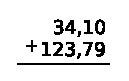
\includegraphics[width=1.5cm]{frac1}
      \item 
      
      
\includegraphics[width=1.5cm]{frac2}
      \item 
      
      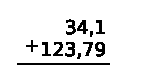
\includegraphics[width=1.7cm]{frac3}
      \item 
      
      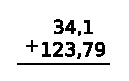
\includegraphics[width=1.5cm]{frac4}
      \end{ChoixQCM}
      \begin{corrige}
     \reponseQCM{ad}
   \end{corrige}
    \end{exercice}
   
\end{GroupeQCM}
\end{QCM}

  


\TravauxPratiques % pour nous "travailler en groupe"

\begin{TP}[]
Voici un extrait de « La Disme », écrit par Simon Stevin en 1585 : \\[0.3em]

« Les 27 \circled{0} 8 \circled{1} 4 \circled{2} 7 \circled{3} donnés, font ensemble 27 $\dfrac{8}{10}$, $\dfrac{4}{100}$, $\dfrac{7}{1\,000}$, ensemble 27 $\dfrac{847}{1\,000}$, et par même raison les 37 \circled{0} 6 \circled{1} 7 \circled{2} 5 \circled{3} valent 37 $\dfrac{675}{1\,000}$. Le nombre de multitude des signes, excepté \circled{0}, n'excède jamais le 9. Par exemple nous n'écrivons pas 7 \circled{1} 12 \circled{2}, mais en leur lieu 8 \circled{1} 2 \circled{2}. »

\partie{Simon Stevin}

Par groupe, en vous documentant, répondez aux questions suivantes.
\begin{enumerate}
 \item Où Simon Stevin a-t-il vécu ?
 \item Quels sont les domaines dans lesquels Simon Stevin a travaillé ? Faites la synthèse des réponses de chaque groupe.
 \end{enumerate}
 
\partie{La Disme} % Pourquoi cette ligne est si rentrée ?

\begin{enumerate}
\item Cherchez comment on écrit de nos jours le nombre 38 \circled{0} 6 \circled{1} 5 \circled{2} 7 \circled{3}.

Comparez avec les réponses des autres groupes.

\item Écrivez, à la manière décrite par Simon Stevin, les nombres $124 + \dfrac{7}{10} + \dfrac{5}{100}$ et 34,802.

Comparez avec les réponses des autres groupes.

 \item Choisissez trois nombres décimaux différents et écrivez-les à la manière décrite par Simon Stevin.
 \item échangez ensuite avec un autre groupe ces nombres écrits à la manière de Simon Stevin. Cherchez alors comment on écrit de nos jours les nombres que vous avez reçus.
 \item Faites une recherche pour trouver les différentes notations utilisées depuis 1585 pour l'écriture des nombres décimaux.
 \end{enumerate}
\end{TP}

%%%%%%%%%%%%%%%%%%%%%%%%%%%%%%%%%%%%%%%%%%%%%%%%%%%%%%%%%%%%%%%%%%%%%%%%%%%

\begin{TP}[Compétitions dans la classe]
Préparatifs : fabriquez une étiquette de carton pour chaque élève de la classe, comportant son nom et son prénom. Mélangez ces étiquettes.

Voici un exemple de liste de calculs à effectuer :
\begin{enumerate}
 \item $853,12 + 19,7$ ;
 \item $538,21 - 42,16$ ;
 \item $65,24 \cdot 7,38$ ;
 \item $68,37 \div 3$.
 \end{enumerate}

\partie{Entraînement en individuel (appelé 1 contre 10)}
Pour chaque manche, un élève $A$ est tiré au sort à l'aide des étiquettes et passe au tableau où un seul calcul écrit est à effectuer. \\[0.5em]
L'élève $A$ l'effectue en public pendant que tous les autres cherchent chacun sur une feuille. \\[0.5em]
Dès qu'un élève a trouvé la réponse et a écrit le calcul, il lève la main. Le professeur surveille le tableau et circule dans la classe pour vérifier le travail de chaque élève. \\[0.5em]
Il compte à haute voix de 1 à 10 en ajoutant 1 chaque fois qu'un travail est considéré comme correct. \\[0.5em]
Arrivé à 10, si l'élève $A$ n'a pas trouvé, la classe a gagné la manche. Par contre, si l'élève $A$ trouve avant la fin du décompte à 10, c'est lui qui a gagné.

\partie{Par équipes (appelé 2 contre 5)}
On constitue des binômes équilibrés d'élèves.\\[0.5em]
Lors du tirage au sort, l'élève $A$ désigné passe au tableau accompagné de son coéquipier mais seul l'élève $A$ peut écrire. \\[0.5em]
On démarre la compétition comme dans le « 1 contre 10 » mais le professeur ne compte que jusqu'à 5. 
\end{TP}

\newpage


\pagebreak

\Recreation
\begin{enigme}[La constante de Champernowne]

Ce nombre, inventé par le mathématicien anglais David Gawen Champernowne en 1933, commence par

0,123456789101112131415 \ldots . \\[-1em]
\begin{enumerate}
 \item Quelle est la particularité de cette constante ? Donne les dix décimales suivantes.
 \item Quelle est l'arrondi, au cent-milliardième près, de cette constante ?
 \end{enumerate}
 \end{enigme}
        
\vspace*{2em}
        
\begin{enigme}[Défis]
Combien de fois faudrait-il utiliser le chiffre 1 si l'on voulait écrire tous les nombres entiers de 1 à 999 ? Et le chiffre 9 ?

Donne le nombre de mots utilisés pour écrire tous les entiers plus petits que 100.
 \end{enigme} 
 
 \vspace*{2em}

\begin{enigme}[Calculatrices infernales 1 (d'après Apmep)]
Sur la calculatrice d'Aïsha, la touche pour afficher la virgule ne fonctionne plus et la touche « $=$ » ne peut fonctionner qu'une seule fois par ligne de calcul.

Comment peut‑elle trouver le résultat de $(17,32 \times 45,3) + 15,437$ ?
 \end{enigme} 
 
 \vspace*{2em}

\begin{enigme}[Calculatrices infernales 2 (d'après Apmep)]
Bruce vient de faire tomber sa calculatrice. Elle ne comporte plus que les chiffres, la virgule et les quatre opérations, mais quand on appuie sur « $+$ » elle ajoute 1, quand on appuie sur « $-$ » elle retranche 1, quand on appuie sur la touche « $\times$ » elle multiplie par 10 et quand on appuie sur la touche « $\div$ » elle divise par 10. \\[-1em]
\begin{enumerate}
 \item Romain emprunte la calculatrice de Bruce. Il tape 27,2 puis appuie ensuite sur les touches « $\times$ », « $\times$ », « $+$ », « $+$ », « $-$ », « $\div$ », « $\div$ », « $\div$ », « $+$ », « $\times$ ». Quel résultat Romain trouve-t-il ?
 \item Comment peut‑il passer en sept opérations :    
 \begin{colitemize}{3}
  \item de 3,14 à 300 ?
  \item de 3,14 à 297 ?
  \item de 297 à 0,2 ?
  \end{colitemize}
 \item Tu viens de passer de 3,14 à 0,2 en quatorze opérations. Trouve un chemin qui permette de faire cela avec le minimum d'opérations. Compare avec tes camarades ; \\[0.5em]
Trouve un chemin qui permette de passer de 5 à 4,99 en un minimum d'opérations puis compare avec tes camarades.
 \end{enumerate}
\end{enigme} 



